%Review of existing harmonic excitation.
%	Nonlinear Systems
%		Traditional Metrics (THD, IMD)
%		Minimisation of Nonlinear Distortion
%		Advent of "Nonlinear Niceness"
%	Timbre of nonlinear distortions (Martens and Marui type shit)
%	Uses of Harmonic Excitation
%	Harmonic Generation Methods
%		Static Nonlinearities
%		Bandwidth Extension (high frequency reconstruction)
%		Individual Harmonic Generation (SMC paper)
%		Psychoacoustic Enhancers

\chapter{Harmonic Excitation}

\section{Intro}
	\note{Harmonic excitation is of the chain. Look I wrote a paper about it \citep{Enderby2013Methods}.}

\section{Nonlinear Systems}
	\note{THD and IMD are rubbish but served some purpose in the olden days. Some more metric were made but they were
	      still only concerned with minimising distortion. Then some bloke decided distortion was cool.}

\section{Timbre of Nonlinear Distortion}
	\note{Martens and Marui got all up in that shit.}

\section{Uses of Harmonic Excitation}
	\note{Not really sure what this bit is for yet.}

\section{Harmonic Generation Methods}
	\note{I like to generate harmonics, basically a nonlinear process}

	\subsection{Static Nonlinearities}
		\note{DAFx Paper}

	\subsection{Bandwidth Extension}
		\note{Look at Figure \ref{fig:SpectralFolding} 'aint it fancy.}
		\begin{figure}[h!]
			\centering
			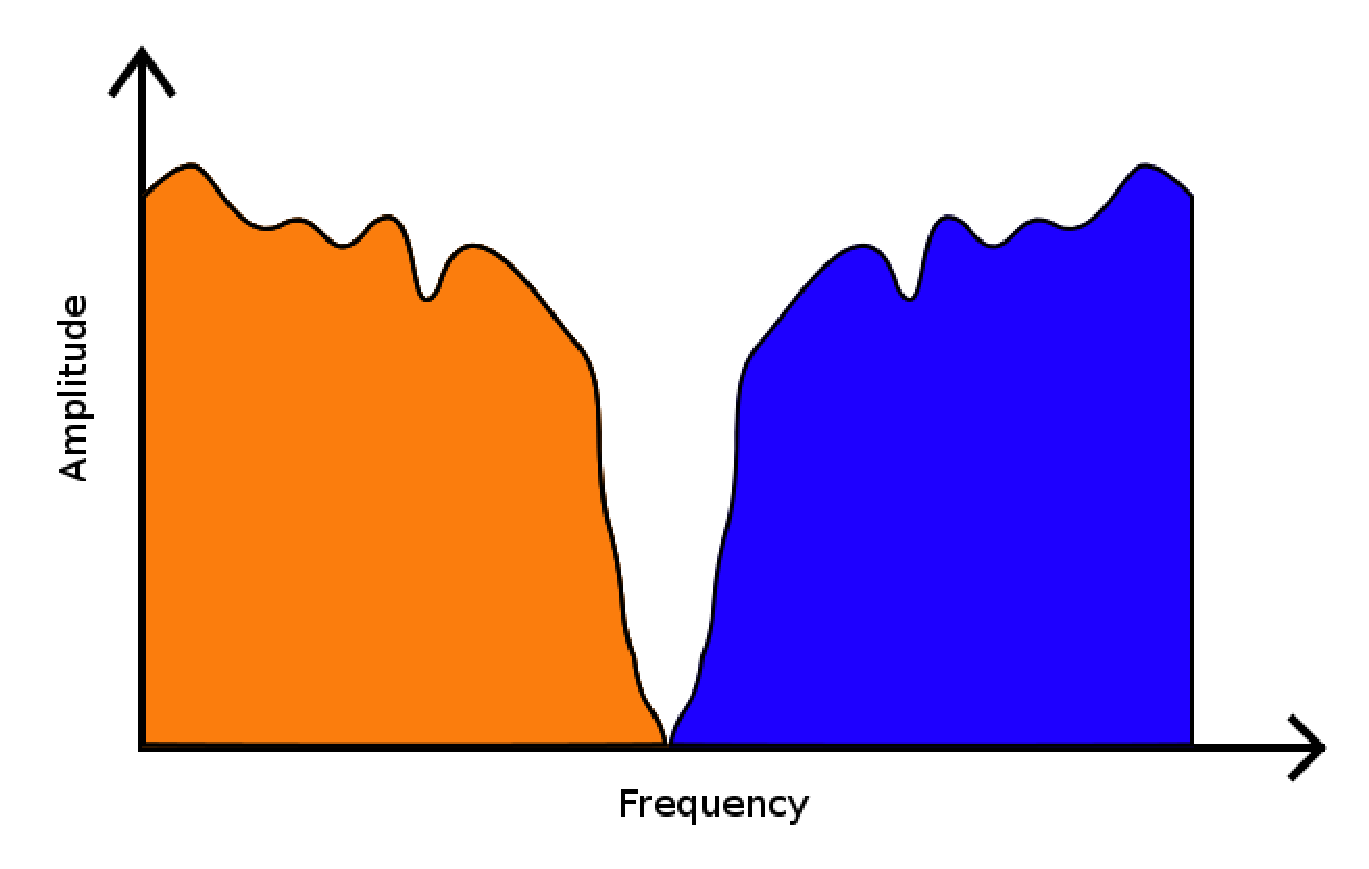
\includegraphics[width=0.5\textwidth]{Chapter3/Images/SpectralFolding.eps}
			\caption{Spectral Folding}
			\label{fig:SpectralFolding}
		\end{figure}

	\subsection{Individual Harmonic Generation}
		\note{SMC paper}

	\subsection{Psychoacoustic Enhancers}
		\note{Probably the most well known perceptual control effects out there.}
